\chapter{Heisenberg model of magnetism\label{sec:xxz}}
\thispagestyle{chapterBeginStyle}
    It is well known, that we can divide magnetic materials into two broad groups: those which
exhibit magnetic properties in reaction to external magnetic field and those which have a nonzero
magnetic moment without external field~\autocite{spalek2015}. First group consists of paramagnetic
and diamagnetic systems. In the former, nonzero net magnetic moment comes from alignment of
valence electrons' spins in the direction of external magnetic field. In the latter, we deal with
 an inductive effect in which external field induces magnetic dipoles opposing the field tha have
induced them. Diamagnetism exists in all materials, however it is usually much weaker than other magnetism related
effects and thus only detectable in the absence of them. Second group includes ferromagnets, which
exhibit spontaneous magnetization below Curie temperature, and ferrimagnets, which are 
composed of two ferromagnetic sublattices with different spontaneous magnetization. There
are also antiferromagnets, which are essentially a special case of ferrimagnets in which the two sublattices,
below the so-called N{\'e}el temperature, have spontaneous magnetizations of equal magnitude
but opposite directions~\autocite{nolting2018theoretical}.

There are two paradigmatic models of magnetism, namely the Heisenberg model, which describes magnetism
of localized electrons and their magnetic moments (spins), and the Hubbard model which deals with
magnetism of delocalized electrons, called the itinerant magnetism. In this thesis we will focus on
a special case of the former of two models, namely the XXZ model.


\section{Heisenberg-Dirac exchange interaction}
We will now proceed with a derivation and a physical motivation of Heisenberg model.
Our discussion will be based on the books by~\textcite{spalek2015} and 
thesis by~\textcite{Ng2011HeisenbergM}.
The story begins with two electrons interacting with each other via Coulomb potential.
An electron can be described by two quantities, its position in space and its spin.
Two facilitate these two degrees of freedom, we say that \(i\)-th electron's wavefunction
lives in a Hilbert space which is a tensor product of spacial 
wavefunction space \(\mathcal{H}_i \cong L^2(\RR^3) \otimes \mathfrak{h}_i \), where
\(L^2(\RR^3)\) is the usual space of square-integrable functions on \(\RR^3\),
and spin wavefunctions space \(\mathfrak{h} \cong \CC^2\) is a two-dimensional vector space spanned by
\(\ket{\ua} = \binom{1}{0} \) and \(\ket{\da} = \binom{0}{1}\).
The combined wavefunction of a composite two-particle system it then an element of
\(\mathcal{H}_1 \otimes \mathcal{H}_2\), which can be decomposed into spacial and spin
components, i.e\ \(\mathcal{H}_1 \otimes \mathcal{H}_2 \cong\mathcal{H}_{\mathrm{space}} 
\otimes \mathcal{H}_{\mathrm{spin}}\), where \(\mathcal{H}_{\mathrm{space}} 
\cong L^2(\RR^3) \otimes L^2(\RR^3)\) and \(\mathcal{H}_{\mathrm{spin}} \cong
\mathfrak{h}_1 \otimes \mathfrak{h}_2\). 

Hamiltonian of two interacting electrons is given by:
\begin{equation}
    H_C = \underbrace{-\frac{\hbar^2}{2m} \laplacian_1  
    -\frac{\hbar^2}{2m} \laplacian_2 }_{\textrm{free particles}}
     + \underbrace{V(\bm{r}_1,\bm{r}_2)}_{\textrm{interaction}}
     \label{eq:Coulomb Hamiltonian}
\end{equation}
where in case of Coulomb interaction we have \(V(\bm{r}_1,\bm{r}_2)=\frac{e^2}
{\abs{\bm{r}_1-\bm{r}_2}}\).
Formally, this Hamiltonian acts on the space \(\mathcal{H}_1 \otimes \mathcal{H}_2\).
However, it depends only on the spatial coordinates \(\bm{r}_1,\bm{r}_2\) and not on
the spin coordinates, so essentially
its actions is restricted to the \(\hspac\) part of the full Hilbert space.
This is a crucial observation that lead to the development of Heisenberg model. We will now
seek a way to replace this Hamiltonian by an equivalent one acting only on 
\(\hspi\).

It is time to invoke the Pauli exclusion principle, which requires the composite wavefunction
of two electrons to be antisymmetric under exchange of pairs of coordinates (both spatial and
spin degrees of freedoms are treated like coordinates). Because 
Hamiltonian~\ref{eq:Coulomb Hamiltonian} does not depend explicitly on spin, the total
wavefunction \(\psi\) can be expressed as tensor product \(\psi_{\mathrm{space}} 
\otimes \psi_{\mathrm{spin}} \). Antisymmetric nature of \(\psi\) then requires one 
of these components to be antisymmetric \((a)\) and the other to be symmetric \((s)\). 
Spatial wavefunctions are of the form:
\begin{align}
    &\spas = \psi_1(\bm{r}_1)\otimes \psi_2(\bm{r}_2) +
    \psi_2(\bm{r}_1)\otimes \psi_1(\bm{r}_2) \\
    &\spaa = \psi_1(\bm{r}_1)\otimes \psi_2(\bm{r}_2) -
    \psi_2(\bm{r}_1)\otimes \psi_1(\bm{r}_2)
\end{align}
where \(\psi_1,\psi_2 \in L^2(\RR^3)\). Spin wavefunctions are elements of \(\CC^2\)
and are given by:
\begin{align}
    &\spis = \ket{\ua\ua},\; 
    \ket{\ua\da} + \ket{\da\ua},\; \ket{\da\da} \\
    &\spia = \ket{\ua\da}-\ket{\da\ua}
\end{align}
where \(\ket{\ua\ua}\) is an usual shorthand notation for \(\ket{\ua}_1 \otimes
\ket{\ua}_2\). Moreover, symmetric spin wavefunctions
constitute a triplet state, whereas antisymmetric one is a singlet state. 

Possible two-electron wavefunctions are thus either \(\varphi=\spas
\otimes \spia\) or \(\chi = \spaa
\otimes \spis\). Expected value of energy of Coulomb interaction 
in these states is given by:
\begin{align}
    &\expectationvalue{H_C}{\varphi} = \expectationvalue{H_C}{\spas} = E^{(s)}\\
    &\expectationvalue{H_C}{\chi} = \expectationvalue{H_C}{\spaa} = E^{(a)} 
\end{align}
Because \(\spaa\) is symmetric with respect to \((\bm{r}_1-\bm{r}_2)\)
we have \(E^{(s)}>E^{(a)}\). Therefore, it is energetically
favourable for our system to pick the total wavefunction that is antisymmetric
in space and symmetric in spin coordinates.

Under the Coulomb interaction, symmetric and antisymmetric spin wavefunctions are not
directly distinguished. It is the difference between spatial parts, together with Pauli
exclusion principle that forces the choice of a triplet state. Let us now do something
similar, but the other way around. We can formally recast the Coulomb Hamiltonian as a
spin-spin interaction acting on \(\hspi\) that would distinguish
between symmetric and antisymmetric spin wavefunctions and thus fix the spatial part.
Let \(\tau^x,\tau^y,\tau^z\) be the \(2\cross 2\) Pauli matrices:
\begin{equation}
\tau^x = \mqty(\pmat{1}),\;\;\;\tau^y = \mqty(\pmat{2}),\;\;\;\tau^z= \mqty(\pmat{3})
\label{eq:Pauli matrices}
\end{equation}
Together with a \(2\cross 2\) identity matrix \(\Id\) they form a basis of vector space of
Hermitian operators acting on a single spin Hilbert space.
They are traceless and of unit determinant. By direct computation it can be checked that
they satisfy a particular commutation and anticommutation relations:
\begin{align}
    &\comm{\tau^j}{\tau^k} = 2 i \varepsilon_{jkl}\tau^{l}\\
    &\anticommutator{\tau^j}{\tau^k} = 2 \delta_{jk} \Id_{2\cross 2}
\end{align}
which in turn leads to the following important property:
\begin{align}
        \comm{\tau^{j}}{\tau^{k}} + \anticommutator{\tau^{j}}{\tau^{k}} 
    &=\left(\tau^{j} \tau^{k}-\tau^{k} \tau^{j}\right)+\left(\tau^{j} \tau^{k}+\tau^{k} 
    \tau^{j}\right) \nonumber \\
    i \varepsilon_{j k l} \tau^{l}+\delta_{j k} \Id_{2\cross 2} &= \tau^{j} \tau^{k}
\end{align}
We define an operator via a formal dot product:
\begin{equation}
    \bm{\tau}_1 \cdot \bm{\tau}_2 = \tau_1^x \otimes \tau_2^x + \tau_1^y \otimes \tau_2^y +
    \tau_1^z \otimes \tau_2^z  
\end{equation}
where subscripts refer to which electron's Hilbert space they act on. 
Let us now examine how this operator acts on \(\ket{\ua\ua}\) spin wavefunction:
\begin{align*}
    \bm{\tau}_1 \cdot \bm{\tau}_2 \ket{\ua\ua} &= 
    \left(\tau_1^x \ket{\ua}_1\right) \otimes \left(\tau^x_2 \ket{\ua}_2\right) + 
    \left(\tau_1^y \ket{\ua}_1\right) \otimes \left(\tau^y_2 \ket{\ua}_2\right) +
    \left(\tau_1^z \ket{\ua}_1\right) \otimes \left(\tau^z_2 \ket{\ua}_2\right)\nonumber\\
    &= \left( \smqty(\pmat{1}) \smqty(1\\0)\right) \otimes \left( \smqty(\pmat{1}) \smqty(1\\0)\right) +
    \left( \smqty(\pmat{2}) \smqty(1\\0)\right) \otimes \left( \smqty(\pmat{2}) \smqty(1\\0)\right)+
    \left( \smqty(\pmat{3}) \smqty(1\\0)\right) \otimes \left( \smqty(\pmat{3}) \smqty(1\\0)\right)\\
    &= \smqty(0\\1) \otimes \smqty(0\\1) + \smqty(0\\i) \otimes \smqty(0\\i) + 
    \smqty(1\\0) \otimes \smqty(1\\0) = \ket{\ua\ua}
\end{align*}
So \(\ket{\ua\ua}\) is an eigenvector of \(\bm{\tau}_1 \cdot \bm{\tau}_2\) with
an eigenvalue \(1\). Carrying out such computations for the three remaining states we get
that all symmetric states are eigenvectors with eigenvalue \(1\), whereas the
antisymmetric state is also an eigenvector, but with eigenvalue \(-3\). 
We could have also obtained this result in a more elegant way by referring directly
to quantum mechanics and algebra of spin angular momentum~\autocite{Sakurai2017}.
If we set \(\hbar = 1\) (which from now on will always be the case), we have the usual
spin vector operators \(\bm{S}_i = \left(\Sx_i,\Sy_i, \Sz_i\right) \) where
 \(S_i^{\alpha} = \tau_i^{\alpha}/2\).
Squares of these operators commute with all other \(S_i^{\alpha}\), hence are the
Casimir operators of their algebras and by Schur's Lemma are proportional to
the identity~\autocite{Woit2017}.
The proportionality constant is equal for spin\(-s\) particles to \(s(s+1)\) and thus
all single spin states are eigenvectors of these operators with eigenvalue \(3/4\). 
We can also construct square of total spin angular momentum operator
\(\bm{S}^2 = (\bm{S}_1 + \bm{2}_2)^2\) for which our triplet (total spin \(S=1\)) and singlet
(total spin \(S=0\)) are eigenvectors with eigenvalue \(S(S+1)\). On the other hand, we 
can calculate \(\bm{S}^2\) directly to obtain the following equation:
\begin{equation}
    S(S+1) = \bm{S}_1^2 + \bm{S}_2^2 + 2\bm{S}_1\cdot \bm{S}_1 = \frac{3}{2} + 2\bm{S}_1\cdot\bm{S}_2
\end{equation} 
Rearranging it, replacing \(\bm{S}_i\) by \(\bm{\tau}_i/2\) and inserting appropriate values
of \(S\) we recreate the previously obtained result on eigenvalues of 
\(\bm{\tau}_1\cdot\bm{\tau}_2\).

After this detour into the world of quantum mechanics of spin, let us return to the problem
at hand. We have established that triplet states and singlet state are eigenvectors of 
\(\bm{\tau}_1 \cdot \bm{\tau}_2\) operators with eigenvalues \(1\) and \(-3\) respectively.
Consider now the following Hamiltonian acting on \(\hspi\):
\begin{equation}
    H_S = \frac{3 E^{(a)} + E^{(s)}}{4} + \frac{E^{(a)} - E^{(s)}}{4} \bm{\tau}_1 \cdot \bm{\tau}_2
    \label{eq:Coulomb recasted}
\end{equation}
It is easy to see that eigenvalues of \(H_S\) are \(E^{(a)}\) for symmetric spin states
(corresponding to \(\spaa\)) and \(E^{(s)}\) for antisymmetric spin state (corresponding to \(\spas\)).
We have thus obtained a Hamiltonian that is equivalent to \(H_C\), yet acting on space 
\(\hspi\) rather than \(\hspac\). Setting \(J = E^{(s)} - E^{(a)}\) and ignoring
constant energy offset, we finally arrive at the Dirac-Heisenberg exchange interaction:
\begin{equation}
    H_S = -\frac{J}{4} \bm{\tau}_1 \cdot \bm{\tau}_2
\end{equation}
or, expressed in terms of usual spin operators:
\begin{equation}
    H_S = -J \bm{S}_1 \cdot \bm{S}_2
    \label{eq:heisenberg dirac}
\end{equation}
Constant \(J\) is called the exchange integral and its sign determines the nature of system described
by this Hamiltonian. If \(J>0\), then symmetric triplet states have lower energy and we say that
the ground state is ferromagnetic. On the other hand, if \(J<0\) then antisymmetric singlet
state has lower energy and the ground state is antiferromagnetic.  

\section{One-dimensional XXZ model}
It now straightforward to generalize this exchange interaction to spins living on an arbitrary
lattice, by summing the spin-disguised Coulomb interaction~\eqref{eq:heisenberg dirac} over all pairs
of spins.
\begin{equation}
    H = -\frac{1}{2}\sum_{i\neq j} J_{ij} \bm{S}_i \cdot \bm{S}_j
    \label{eq:Heisenberg model}
\end{equation}
The factor \(\frac{1}{2}\) is introduced to mitigate double-counting of pairs.
This is the so called Heisenberg (Heisenberg-Dirac) Hamiltonian. What this Hamiltonian
does is describe correlation between spins of single particles located in atoms \(i\) and \(j\)
(lattice sites), induced by repulsive Coulomb interaction. If we were to carry out more formal
second-quantization of original Hamiltonian~\eqref{eq:Coulomb Hamiltonian}, we could have obtained
a more concrete expression for the exchange integral. Assuming that one electron is in a state
described by wavefunction \(\varphi_i(\bm{r}_1)\) and second one in \(\varphi_j(\bm{r}_2)\)
then we would have~\autocite{spalek2015}:
\begin{equation}
    J_{ij} = \int \mathrm{d}^3\bm{r}_1 \mathrm{d}^3\bm{r}_2\; \varphi_i^{\ast}(\bm{r}_1)
    \varphi_j^{\ast}(\bm{r}_2) \frac{e^2}{\abs{\bm{r}_1-\bm{r}_2}}\varphi(\bm{r}_1)
    \varphi_j(\bm{r}_2)
\end{equation}
In practical calculations it is often assumed that electrons are well localized, and thus
the value of this integral falls off quickly enough with increasing distance between them
that only the nearest neighbors interactions are important. Moreover, \(J_{ij}\) is also assumed
to be the same between those nearest neighbors:
\begin{equation}
    J_{ij} = \begin{cases}
        J,\;\;\; i \textrm{ is a neighbor of } j\\
        0,\;\;\; \textrm{otherwise}
    \end{cases}
\end{equation}
These assumptions reduce Heisenberg Hamiltonian to its most popular form:
\begin{equation}
    H = -\frac{J}{2}\sum_{\langle i,j \rangle} \bm{S}_i \cdot \bm{S}_j
\end{equation}
where summation index \(\langle i,j \rangle\) indicates that this sum should be performed over all pairs
of nearest neighbors (with repetitions).

From now on we will be restricting our attention to the case of one-dimensional lattices and
nearest neighbors interaction. First, let us set up the stage. We are interested in studying
a one-dimensional chain of \(L\) spin-\(1/2\) interacting fermions with periodic boundary conditions,
i.e.\ arranged in a circular ring. For visualization of periodic boundary conditions in 
one and two-dimensional cases see Figure~\ref{fig:pbc}.
The underlying Hilbert space is then a \(2^L\)-dimensional
tensor product of \(L\) single spin spaces \(\hspi = \bigotimes_{j=1}^{L}\mathfrak{h}_j\).
To upgrade a single spin operator \(\sigma\) to this product space we will use the
standard embedding:
\begin{equation}
    \sigma_j = \underbrace{\Id_{2\cross 2} \otimes \cdots \otimes \Id_{2\cross 2}}_{j-1}
     \otimes \;\sigma \otimes \Id_{2\cross 2} \otimes \cdots \otimes \Id_{2\cross 2}
    \label{eq:embedding}
\end{equation}
Subscript \(j\) means that even though this operator formally acts on
\(\hspi\), it acts in a nontrivial way only on \(\mathfrak{h}_j\). 

Real world systems usually exhibit some degree of anisotropy, which means that it can
be more difficult to achieve magnetization in one direction than in some other direction.
To capture this behavior, we can slightly generalize the Heisenberg Hamiltonian:
\begin{equation}
    H_{XYZ} = \sum_{j=1}^L  \left( J_{x} \Sx_{j}\Sx_{j+1} + J_{y} 
    \Sy_{j}\Sy_{j+1} + J_{z} \Sz_{j}\Sz_{j+1} \right)
\label{eq:XYZ}
\end{equation}
where periodic boundary conditions are imposed by requiring that \(S^{\alpha}_{L+1} = 
S^{\alpha}_{1}\). Obtained model is known in literature as the XYZ model. However, it is often
the case that a single direction is preferred. We can then choose it to be the \(z\) direction
and set \(J_x = J_y \equiv J \neq J_z \equiv J\Delta\). As a result we get the titular XXZ model:
\begin{equation}
    H_{XXZ} = J\sum_{j=1}^L  \left( \Sx_{j}\Sx_{j+1} + \Sy_{j}\Sy_{j+1} \right) + 
    J\Delta \sum_{j=1}^L \Sz_{j}\Sz_{j+1}
\label{eq:XXZ 2}
\end{equation}
It is convenient to reexpress this model in terms of the so-called spin-flip operators:
\begin{align}
    &S^{+} = \Sx + i\Sy\\
    &S^{-} = \Sx - i\Sy
\end{align}
They get their name from the easily checked fact that \(S^{+}\ket{\da} = \ket{\ua}\) and 
\(S^{-}\ket{\ua} = \ket{\da}\). Inverting these relations:
\begin{align}
    &\Sx = \frac{S^{+} + S^{-}}{2}\\
    &\Sy = \frac{S^{+} - S^{-}}{2i}
\end{align}
and inserting them into~\eqref{eq:XXZ 2} yields:
\begin{equation}
    H_{XXZ} = \frac{J}{2}\sum_{j = 1}^{L}\left( S^{+}_{j} S^{-}_{j+1} + 
    S^{-}_{j}S^{+}_{j+1} \right) + J\Delta\sum_{j = 1}^{L} S^{z}_{j}S^{z}_{j+1}
    \label{eq:XXZ}
\end{equation}
which is the most common form of this Hamiltonian. We could restore the isotropy by setting \(\Delta = 1\),
obtaining yet another version of this model, called the isotropic XXX model. A curious property
of XXX model is that is posses \(SU(2)\) symmetry (rotation of spins), which will be useful for us
in the future. Unless stated otherwise, we will work in units such that \(J = 1\).

Heisenberg model, despite its apparent simplicity, is exceedingly difficult to analyze.
Nevertheless, the one-dimensional XXX version was diagonalized analytically by Hans~\textcite{Bethe1931} 
in 1931, by means of the now famous \textit{Bethe ansatz}. Even more remarkably, Rodney Baxter in
1971 expanded upon the Bethe ansatz and solved the general XYZ model in 
one-dimension~\autocite{Baxter1971,Baxter1972}. However, these solutions, as well as the
so far unsuccessful attempts at solving it in two and more dimensions, are notoriously difficult and
we will not use them in this thesis. Instead, when in need of concrete computations, we will
resort to much simpler numerical methods in form of exact diagonalization~\autocite{Lin1990}.

\begin{figure}[htbp]
    \centering
    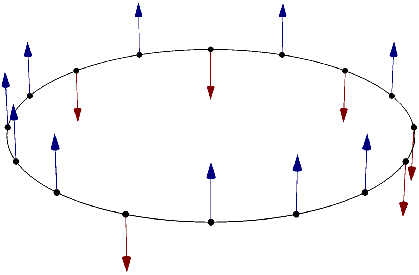
\includegraphics[width=0.8\textwidth]{Figures/ring.pdf}
    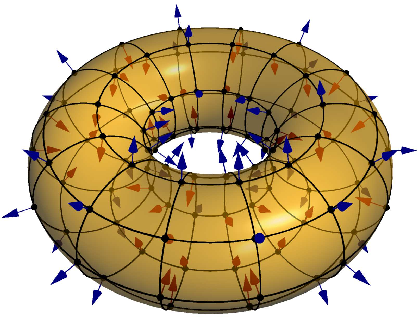
\includegraphics[width=0.85\textwidth]{Figures/torus.pdf}
    \caption{Visualization of periodic boundary conditions in 1-D (circle topology) and
    2-D (torus topology).}
    \label{fig:pbc}
\end{figure}